
\begin{center}

  \textsf{\MakeUppercase{Data visualization workshop}}

\smallskip

\textsf{\MakeUppercase{i320u Information \& Interaction Design}}

\smallskip

\textsf{\MakeUppercase{Dr.~McQuaid}}

\end{center}


\section{Intro}\label{intro}

Go through a Getting Started exercise with Tableau. This comes from the
Tableau website, so you can always go back over this by visiting the
Learning portion of the site.

\begin{center}
  \begin{figure}
    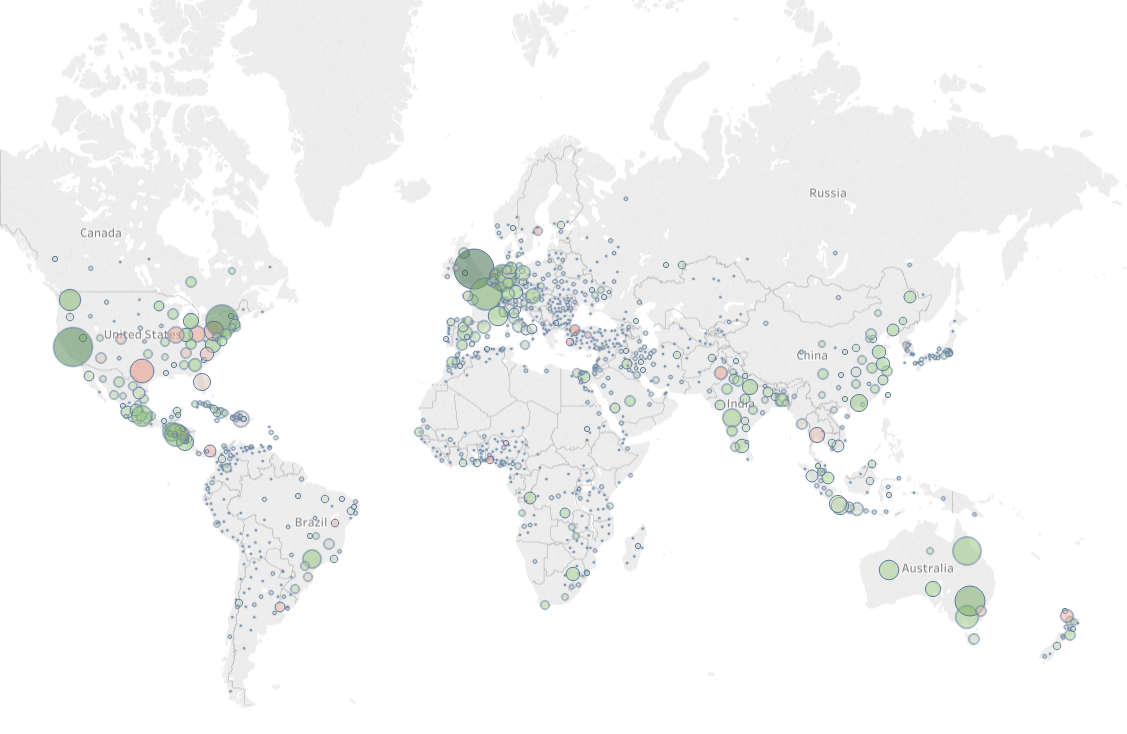
\includegraphics[width=4in]{fiMap.png}
  \end{figure}
\end{center}

\section{Global Superstore}\label{global-superstore}

We'll use an Excel spreadsheet called Global Superstore, shaped as a
table recording orders, returns, and people for a fictional store
operating worldwide. This is \emph{not} the Sample Superstore
spreadsheet! You will quickly get lost if you open the Sample Superstore
spreadsheet!

The Global Superstore spreadsheet is in Canvas \textgreater{} Files
\textgreater{} visualization \textgreater{}
\texttt{Global\ Superstore.xls} so start by downloading it.

\section{Download Tableau}\label{download-tableau}

Next, download a trial copy of Tableau. Students can obtain a special
license for free but don't worry about that right now. The trial copy
will serve our purposes.

\section{Open the application}\label{open-the-application}

\begin{itemize}
\item
  The first thing you should see is a screen with headings including
  Connect and Open and Discover.
\item
  Look at More Servers briefly. This shows the range of data sources you
  can use.
\item
  Return to the main screen.
\end{itemize}

\section{Open the Global Superstore
spreadsheet}\label{open-the-global-superstore-spreadsheet}

\begin{itemize}
\item
  Choose Excel from the Connect pane. Double-click on the Global
  Superstore spreadsheet to select it.
\item
  Now you're in the Data Connection window. From here, you can see that
  there are three worksheets in the Excel file, Orders, People, and
  Returns.
\end{itemize}

\section{Choose the Orders worksheet}\label{choose-the-orders-worksheet}

\begin{itemize}
\tightlist
\item
  Drag Orders to the Canvas, which is the large white rectangle. You
  will see the first few rows of that worksheet, which is organized as a
  table with each row representing information about a particular order
  and each column representing an attribute. This is the way a database
  table would be laid out.
\item
  You can now join this table to one of the other tables by dragging
  Returns to the canvas. This will reveal a path between the two tables.
  You can select a way to join these tables together using the dialog at
  the bottom of the screen.
\item
  Throughout the rest of this tutorial, though, we are going to only use
  Orders. Click Remove from the options triangle on the Returns icon.
\item
  Look at the preview of the data in the lower part of the screen. You
  can click on each name to rename it. Click on the icon \texttt{\#}
  beside the Row ID and change the data type from integer (whole number)
  to string.
\item
  Another thing you can do is to break up a piece of data into its
  parts. The Order ID, for instance, includes a two letter code for the
  distribution center as well as four digits for the year and an integer
  for the productid. Create a separate column for distribution center
  with the following steps. (1) Click on the options triangle and select
  split. (2) Delete the Split 2 column and the Split 3 column. (3)
  Rename the Split 1 column as Distribution Center. (Note that the split
  columns show up at the end of the list of columns!)
\item
  In the upper right screen corner, you can choose whether the
  connection to the spreadsheet is live or if, instead, you extract the
  data in the spreadsheet into Tableau. Leave it live for now but be
  aware that, if you are connected to an enterprise database, you may
  reduce server load by extracting data.
\end{itemize}

\section{Go to the Tableau worksheet}\label{go-to-the-tableau-worksheet}

\begin{itemize}
\tightlist
\item
  Click on the Sheet 1 tab at the bottom of the screen. This is where
  you will do the main work.
\item
  Look at the parts of the screen. There is a ribbon at the top, a data
  pane on the left, the main workspace in the center, and a show me pane
  on the right. Above the main workspace and below the ribbon are two
  shelves: Columns and Rows.
\item
  The data pane contains two kinds of data: categorical and numeric. The
  numeric items are called \emph{Measures}. Earlier versions of Tableau
  called the categorical items \emph{Dimensions} so you may see that
  term from time to time. The two parts of the data pane are separated
  by a horizontal line between the categorical items and the numeric
  items.
\end{itemize}

\section{Create a data visualization}\label{create-a-data-visualization}

\begin{itemize}
\tightlist
\item
  Drag the word Category from the Dimensions part of the data pane to
  the Rows shelf. You should see three rows representing the categories
  in Sheet 1.
\item
  Drag Quantity from the Measures part of the data pane to the Columns
  shelf. You should see sideways barchart of of Quantity by Category in
  Sheet 1.
\item
  Drag Segment from Dimensions to Rows. The barchart expands with three
  segments per category: Consumer, Corporate, and Home Office.
\item
  Drag Market from Dimensions to Columns. The barchart expands into
  seven smaller barcharts, one for each market.
\item
  Drag Market again, this time from Dimensions to Color in the Marks
  shelf. Now each barchart is colored according to its market.
\end{itemize}

\section{Look around}\label{look-around}

The items you dragged into the Columns shelf and Rows shelf are called
Pills in Tableau parlance. Notice that the Measures pill, SUM(Quantity),
is colored green while the Dimensions pills are all colored blue. The
measures pill represents a number in a more or less continuous
distribution, while the dimensions are categorical, in more or less
discrete distributions.

\section{Clear sheet}\label{clear-sheet}

In the ribbon, select the Clear Sheet icon. It has a tiny barchart,
partly covered by an \(\times\).

\section{A new visualization}\label{a-new-visualization}

\begin{itemize}
\tightlist
\item
  Drag Sales from Measures into the left margin of Sheet 1. A single bar
  appears, showing the sum of sales for the Global Superstore to be
  about 12.6 million.
\item
  Drag Order Date from Dimensions into Columns. The barchart
  auto-converts into a line chart showing sales over time and labeled by
  Year.
\item
  Click the \(+\) symbol on the left of the YEAR(Order Date) pill. The
  line chart expands into four line charts, one for each year, and
  aggregated at the quarter level.
\item
  Swap the positions of the two blue pills in Columns so that Quarter is
  in front of year. Now the view is changed so that each line chart
  shows one quarter over four years.
\item
  Drag the YEAR(Order Date) pill out of Columns and onto Color on the
  Marks shelf. Now the years are in one stacked line chart.
\item
  Click on the options triangle of the QUARTER(Order Date) pill. Click
  on Months to expand the stacked line chart according to months.
\item
  Click on the options triangle of the SUM(Sales) pill. One of the
  choices there is Measure(Sum). Click there and you can see some other
  choices of Measures. Click on Average to see how that will look.
\item
  Then click on Sum to return to the previous view. (Or click Undo.)
\item
  Click on the options triangle of the SUM(Sales) pill again. This time,
  go to Quick Table Calculation and look at the submenu.
\item
  Choose Year over Year Growth from the submenu. The line chart changes.
\item
  Drag Sales from the Measures pane back into Rows and now you have two
  displays.
\item
  Now move the SUM(Sales) that represents Year over Year Growth from
  Rows to the Tooltip in the Marks shelf. Now the Year over Year Growth
  line chart disappears and, instead, year over year growth is shown as
  a tooltip when you hover over points in the remaining chart.
\item
  Drag Category to the Rows shelf. Now the line chart is split into
  three charts, one for each category.
\item
  The peak for office supplies in August reflects the annual back to
  school sale. Annotate the chart with that fact.
\item
  Right click near that point and choose Annotate, Area from the
  resulting menu. Write in an annotation like ``This is our annual back
  to school sale.'' Click OK. If the annotation background is hiding
  part of the line, you can move it or decrease its shading on the
  format menu.
\item
  Right click on the Sheet 1 tab at the bottom of the screen and rename
  this ``Sales Seasonality.''
\end{itemize}

\section{Create a spreadsheet from the
visualization}\label{create-a-spreadsheet-from-the-visualization}

Right click anywhere in the chart and choose Copy, Data from the
resulting menu. If you open a copy of Excel you can paste it into a new
workbook, where it will include the Year over Year growth calculation
from the tooltips.

\begin{itemize}
\tightlist
\item
  Instead of exporting to Excel, you can view the data by going to the
  menu and choosing Worksheet \textgreater{} Duplicate as Crosstab
\item
  Switch to the new tab, Sales Seasonality (2)
\item
  Click on the Swap Rows and Columns icon in the ribbon so that months
  are rows.
\item
  Move Category from the Columns shelf to the Rows shelf.
\item
  Click on Standard on the ribbon and choose Entire View to make the
  crosstab take up the entire window space.
\item
  Drag Profit from Measures to Color in the Marks shelf.
\item
  Make the colors stand out more by clicking Color on the Marks shelf
  and choosing Edit Colors.
\item
  Choose Red-Green Diverging, Use Full Color Range, and Stepped Color
  with 6 steps.
\item
  Choose Undo on the ribbon and try a different way to emphasize
  profitability.
\item
  Click the options triangle for the Marks shelf. It currently reads
  Automatic. Change it to Square. Now you just see colored squares.
\item
  Click on Label on the Marks shelf and choose Show Mark Labels.
\item
  You can change the colors back to red-green diverging if you wish, so
  it looks more like a traditional profit and loss display.
\item
  Double click on the Sales Seasonality (2) tab and rename this
  Crosstab.
\end{itemize}

\section{Create a sheet to explore global sales and
profits}\label{create-a-sheet-to-explore-global-sales-and-profits}

The Crosstab worksheet shows that Furniture is less successful than the
other two categories in the Fall but it does not tell us where the
problem lies. Use a new sheet to try to find the locations of
furniture's profitability problems.

\begin{itemize}
\tightlist
\item
  Click on the New Worksheet icon next to the word Crosstab at the
  bottom of the display.
\item
  Click on the Show Me tab if its window is not already visible. Drag
  the Show Me pane over near the Measures pane.
\item
  Control-click (on Windows) or Command-click (on Mac) on several
  measures and see suggestions for appropriate charts highlight on the
  Show Me pane.
\item
  Select Sales and Country (using Control-click if on Windows or
  Command-click if on Mac). One of the highlighted types is the symbol
  map. Select that. You should see a world map with dots of different
  sizes centered on Country territories. If not, drag Country and Sales
  to the map. They should appear as pills on the Marks shelf.
\item
  Drag State onto the map and notice that the Sales circles are now
  broken down into smaller regions.
\item
  Drag the Size slider on the Marks shelf to increase the size of the
  dots.
\item
  Choose Color on the Marks shelf and adjust the opacity to around 50
  percent.
\item
  Also on Color add dark blue borders instead of leaving them set at
  Automatic.
\item
  There should be a size legend beside the display. Click on it so the
  options triangle appears and select Hide Card on that menu.
\item
  Drag Profit to Color. You may want to change the colors to Red-Green
  diverging.
\item
  Search for United Arab Emirates using the magnifying glass on the map.
  The map should zoom into UAE. Select the pin icon to \emph{unpin} the
  map, zooming out to the previous view.
\item
  Drag Category to the Filter shelf. Choose Furniture in the dialog box.
  Now the map is restricted to showing profitability and sales of
  furniture. The color of the circles represents profit and the size of
  the circles represents sales.
\item
  Right click the Category: Furniture pill and choose Show Filter on the
  resulting menu. Now anyone viewing the exported visualization can
  choose a category or categories of interest.
\item
  Restrict the viewer's choice by clicking the options triangle on the
  Category filter. Currently \texttt{Multiple\ Values\ (list)} is
  checked. Change that by clicking \texttt{Single\ Value\ (list)}. Now a
  viewer can only choose one category at a time.
\item
  Rename this sheet Global Sales and Profits.
\end{itemize}

\section{Create a sheet to explore
sub-categories}\label{create-a-sheet-to-explore-sub-categories}

Click on New worksheet.

Furniture is doing poorly but what types of furniture are dragging the
category down? One way to find out is to explore the sub-categories
under the Furniture category.

Try the Show Me method again to identify a promising chart type for the
columns of interest: Category, Sub-Category, and Sales. Remember you
must control-click (Windows) or command-click (Mac) the columns of
interest after first revealing the Show Me pane.

\begin{itemize}
\tightlist
\item
  Click on several of the Show Me suggestions to see what they would
  look like.
\item
  Finally, choose \emph{Horizontal Bars} from Show me and close the Show
  Me pane.
\end{itemize}

You know that there is a hierarchical relationship between Category and
Sub-Category. Tableau has a technique for expressing that relationship
in a way that you can drill down from the more general to the more
specific. This technique is to drag and drop columns on top of each
other in the data window.

\begin{itemize}
\tightlist
\item
  Drag Sub-Category on top of Category in the Dimensions part of the
  Data pane. A \emph{Create Hierarchy} dialog box appears. Name the
  hierarchy \emph{Products} in that dialog box. It now appears in
  Dimensions with a hierarchy symbol beside it.
\item
  Drag Product Name onto the Products hierarchy.
\item
  Now use the plus and minus on the Category pill to expand and contract
  the hierarchy.
\item
  You will also find that there are pluses and minuses you can
  manipulate in the same way inside Sheet 4.
\item
  Make sure that both categories and subcategories are visible when you
  are done exploring the pluses and minuses.
\item
  Swap the axes using the same Swap Rows and Columns icon on the ribbon
  you used before.
\item
  Use the Standard button on the ribbon to resize the chart to Entire
  View.
\item
  Click the Category pill. Then click the Sort Descending button in the
  ribbon. Now Technology is on the left, followed by Office Supplies.
  Technology has the most total sales, followed by Office Supplies.
\item
  Click on the tiny barchart icon on the left side of the barchart,
  adjacent to the word Sales. When you click it repeatedly, it changes
  the sort order of the sub-categories within categories, without
  changing the categories.
\item
  Choose Show Mark Labels from the menu to display the sales for each
  bar. Then choose it again to hide them.
\item
  Drag Profit to Color and observe that Tables are a significant profit
  problem in the Furniture category despite their sales volume.
\item
  Drag Market to the left of Sheet 4. A dashed vertical line should
  appear and, when you release the mouse, barchart should expand into
  seven small charts, one for each market. You can see that Table
  profitability is a problem in four of the seven markets.
\item
  Group some of the office supply columns together. Select the captions
  for all but the first three by shift-clicking. In the dialog box that
  appears, select group members.
\item
  Rename the aggregated category by clicking its caption and selecting
  Edit Alias from the resulting menu. Call it ``small office supplies.''
\item
  Simplify the view. Swap the axes, change Fit to Standard, remove
  Market from the Columns shelf, and hide the field labels for Category
  and Sub-Category by right clicking on either of them and selecting
  ``Hide Field Labels for Rows.''
\item
  Rename this sheet Sales by Category.
\end{itemize}

\section{Create a sheet to explore shipping
cost}\label{create-a-sheet-to-explore-shipping-cost}

Suppose you have a hunch that the low profitability in furniture is
related to shipping costs. Now create a new sheet to explore that
possibility.

\begin{center}
  \begin{figure}
    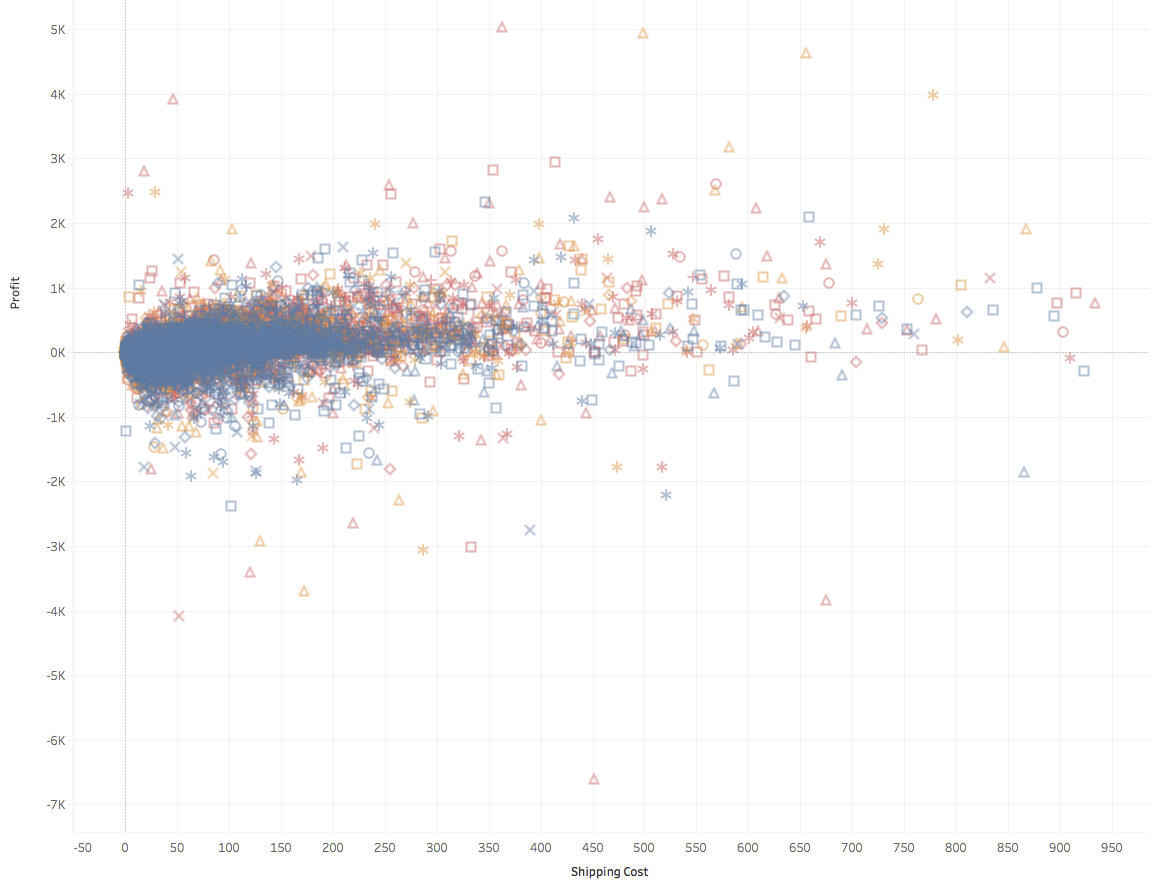
\includegraphics[width=4in]{fiShippingCost.png}
  \end{figure}
\end{center}

\begin{itemize}
\tightlist
\item
  Select New Worksheet.
\item
  Drag Profit to the Rows shelf.
\item
  Drag Shipping Cost to the Columns shelf.
\item
  Drag Market onto the Shape shelf.
\item
  Drag Category onto the Color shelf.
\item
  Drag Customer ID onto the Detail shelf.
\end{itemize}

Now Tableau makes a mark for each customer, shaped by Market and colored
by Category. (There may actually be more than one mark per customer if a
customer has ordered from more than one category or in more than one
market.) Each mark represents the sum of profit and shipping cost per
customer per market per category.

\begin{itemize}
\tightlist
\item
  Click on the Analysis menu tab at the top of the window. Notice that
  \emph{aggregate measures} is checked. Uncheck it and now there is a
  single mark for each transaction. Any transactions below the
  horizontal 0K line are not profitable!
\item
  On the Marks shelf, click to the left of Customer ID and select Label.
  Now the Customer ID labels each point. Go back to that same menu and
  select Detail or click Undo.
\item
  Another way to label is to drag something onto label, for example,
  drag Sales onto the Label shelf.
\item
  Click the Label shelf and click the three dots next to Text. An edit
  label dialog appears. Add a dollar sign before the angle brackets
  surrounding sales. Now the labels will display in dollars.
\item
  Add trend lines. Switch from the data pane on the left to the
  Analytics pane.
\item
  Select Trend line from the Analytics pane and drag it onto Sheet 5.
  When it is over Sheet 5 a menu appears. Drag the Trend Line to the box
  marked Linear. Notice that three trend lines appear, one for each
  category. Observe that the Furniture line shows that profits rise less
  with shipping costs than do the profits in the other two categories.
\item
  Look at the mark for one of the low profit / high shipping cost
  transactions. A tooltip appears.
\item
  Click on the point. A menu appears on the tooltip. Select View Data on
  the tooltip. A new panel appears with a summary. Click on Full Data
  and look at the details of the transaction. Close the window.
\item
  Remove Sales from the Marks shelf. The numbers vanish.
\item
  Right click in Sheet 5 and uncheck Show Trend lines.
\item
  Call this sheet Customer Breakdown.
\end{itemize}

\section{Compile a dashboard to
share}\label{compile-a-dashboard-to-share}

A dashboard is the Tableau way to share multiple views of data. You can
integrate each of the sheets you've created into a single dashboard to
tell a story of data exploration.

\begin{itemize}
\tightlist
\item
  Click on the New Dashboard icon at the bottom of the window.
\item
  Click on the options triangle beside size and choose Laptop Browser,
  \(800 \times 600\).
\item
  Notice that all the sheets you created are listed on the left and you
  can hover over them to see a preview.
\item
  Drag Global Sales and Profits into the view.
\item
  Drag Sales by Category into the bottom half of the view.
\item
  Drag Customer Breakdown into the bottom right quadrant of the view.
\item
  In both cases, Sales by Category and Customer Breakdown, make sure Fit
  is set to Entire View. Right click on the panel, then use the More
  Options triangle on the tab to find the Fit option.
\item
  Right click on the Dashboard tab and rename it Sales Dashboard.
\item
  Add the name to the dashboard itself by clicking Show dashboard title
  in the lower left corner.
\item
  Edit the title by double-clicking it, bringing up an edit dialog.
\item
  In the dialog, change the size of the title from 18 to 16 and center
  it. Click OK to accept your changes.
\item
  Click on the Category menu in the upper right to change the map.
  Suppose, though, that you want all three visualizations to change to
  the selected categories?
\item
  Right click on the Category panel and choose Apply to Worksheets from
  the menu. Choose All Using This Data Source from the submenu. Now all
  three visualizations change according to the selection.
\item
  Click on the red mark over Auckland, NZ. Suppose you would like to
  know more about that state. On the map's tab, choose More Options.
  From the menu, choose Use as Filter. Now you can click on any circle
  in the map and see the related info in the other two visualizations.
\end{itemize}

\section{Create story points}\label{create-story-points}

Another way to view the visualizations you have created is through what
Tableau calls \emph{story points}. This consists of a navigator bar over
a series of visualizations. By clicking on the navigator bar, you step
through the story points, capturing each visualization at a specific
point.

\begin{itemize}
\tightlist
\item
  Click on the New Story icon.
\item
  Change the size to Laptop Browser \(800 \times 600\).
\item
  Drag Global Sales and Profits onto the view.
\item
  Add a caption, saying ``Overall, our profits look strong''.
\item
  Note that the visualization is still interactive. Test that by
  selecting categories.
\item
  Click on Furniture on the Category panel. A menu appears above the
  caption. Select Save as New.
\item
  Add a new caption, ``But not across all categories''.
\item
  Drag the \emph{Drag to add text} rectangle onto the visualization.
\item
  Add the text ``Furniture appears to have poor profitability in some
  areas'' and resize the text to 12.
\item
  Double click on Sales by Category to create a third story point. Add
  the caption ``Here's the biggest problem''.
\item
  Again add a callout by dragging the \emph{Drag to add text} rectangle
  to the bottom of the view. Say ``Tables are dragging down Furniture's
  profits.''
\item
  Drag the Sales Dashboard to the right of the list of captions and add
  it as a fourth story point.
\item
  Notice that the Sales Dashboard does not fit very well.
\item
  Click on the Go To Sheet icon to the right of the Sales Dashboard's
  name in the Story pane.
\item
  Resize it to ``Fit to Story''. Also take off the Sales Dashboard
  title.
\item
  Now return to the Story 1 window and notice that it fits better.
\item
  Add a caption ``What's behind it? Next steps \ldots{}''
\item
  Click on Furniture on the Category panel and then select Update from
  above the caption.
\item
  Double click on Story 1, bringing up an edit dialog.
\item
  Rename it to ``Profitability: The Whole Story''.
\item
  Save it as a packaged workbook. Give it a filename of
  \texttt{globalSuperstore.twbx}. Since it is a packaged workbook you
  will not need the separate spreadsheet file
  \texttt{Global\ Superstore.xls} to work with it.
\end{itemize}

\begin{center}
  \begin{figure}
    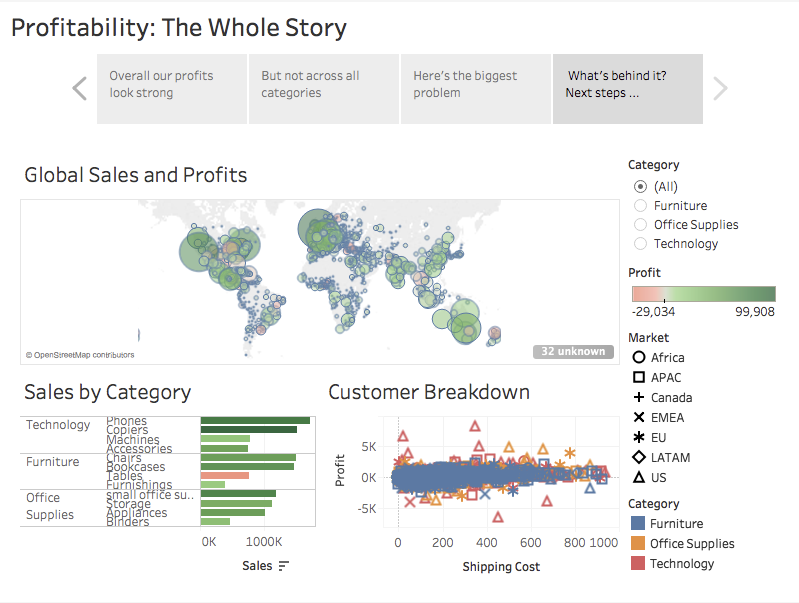
\includegraphics[width=4in]{fiStoryPoints.png}
  \end{figure}
\end{center}

\section{Discussion}\label{discussion}

Now that you have completed an exercise using Tableau your next step
should be to reflect on what you have done. There are a number of
discussion questions to consider.

\begin{enumerate}
\def\labelenumi{\arabic{enumi}.}
\item
  The menu structure of Tableau may change drastically from one version
  to the next. Can you navigate this tutorial in the next (or previous)
  version of Tableau?
\item
  Different chart types are recommended for different types of data. How
  would you characterize these chart types? What is it about the data
  that leads to the recommendations?
\item
  Is Tableau biased in any way? Is it easier to make some kinds of
  arguments with Tableau than others?
\item
  Tableau accepts live data and allows you to connect your visualization
  to live, changing data. Suppose the point you are trying to make is no
  longer supported by data in future. Will you be blamed for that
  change?
\item
  Tableau makes a lot of default choices that you changed. Do you think
  it could (or should) learn your preferences over time? What would it
  take to do that?
\item
  What is a data visualization? What would have to be subtracted from
  these pictures so that they could not be called data visualizations?
\end{enumerate}
